(would be cool here to have just a picture you took of speckle)
\begin{figure}[ht]
\centering
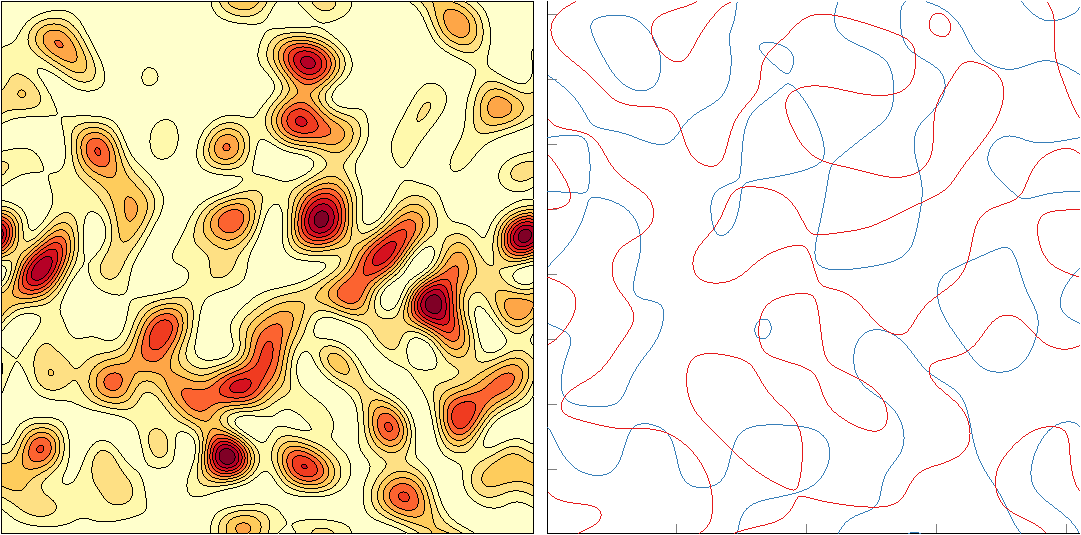
\includegraphics[keepaspectratio,width=15cm]{speckle/figures/introfig.pdf}
% ~/getvortex/specklefield.m
% make the colorbars below
\caption{Paragon speckle field, produced by the Fourier transform method.
								Right: speckle intensity.  Left: contours of the zeros of the real
								and imaginary components of the complex field, intersections of
								which are locations of optical vorticies.}
\label{fig:examplespeckle}
\end{figure}

Under most circumstances, light scattered in to the cone is not homogeneous
but exhibits distinctive intensity fluctuations known as \textit{speckle}.
In optics, this arises due to the interference of coherent waves with
randomly distributed amplitudes and phases.  Speckle in optics is closely
related to the mesoscopic phenomena of universal conductance
fluctuations~\cite{lee1985universal}, and likewise exhibits many of the
same interesting physics such as coherent
backscattering~\cite{akkermans1986coherent}.  This chapter is devoted to
our studies of speckle in the cone.  Here we examine the properties of cone
speckle and compare them with traditional systems.  We also discuss certain
features and correlations which are useful in the context of biosensing.
